%!TEX root = ../template.tex
%%%%%%%%%%%%%%%%%%%%%%%%%%%%%%%%%%%%%%%%%%%%%%%%%%%%%%%%%%%%%%%%%%%%
%% chapter2.tex
%% NOVA thesis document file
%%
%% Chapter with the template manual
%%%%%%%%%%%%%%%%%%%%%%%%%%%%%%%%%%%%%%%%%%%%%%%%%%%%%%%%%%%%%%%%%%%%

\typeout{NT FILE chapter2.tex}%

\chapter{Ultrasound, Transducers and Ultrasound Imaging}
\label{cha:users_manual}

\glsresetall

Fundamental concepts of *what* is an US wave, *how* it propagates and *why* 
does it present different behaviours upon its interaction with different materials 
is discussed in this introductory chapter. The spectral and temporal properties of 
a typical US echo in the two imaging modalities targeted within the scope of this 
dissertation - flow cytometry and 2D/3D B-mode - are also discussed.
This chapter serves as a conceptual basis for justifying the system design premises 
presented in the rest of this dissertation. 

\section{Ultrasound Fundamentals}
\label{sec:ultrasound_fundamentals}

\subsection{Wavefronts}
\label{subsec:ch2_1_wavefronts}

Ultrasound is a mechanical wave that can propagate in a wide variety of 
shapes and *wavefront* morphologies throughout any material medium. It 
can propagate in solids, liquids and, with a little bit more difficulty, 
in gases. If it is a valid matter state, than sound can propagate in it.

\begin{figure}[ht]
     \centering
     \begin{subfigure}[h]{0.3\textwidth}
         \centering
         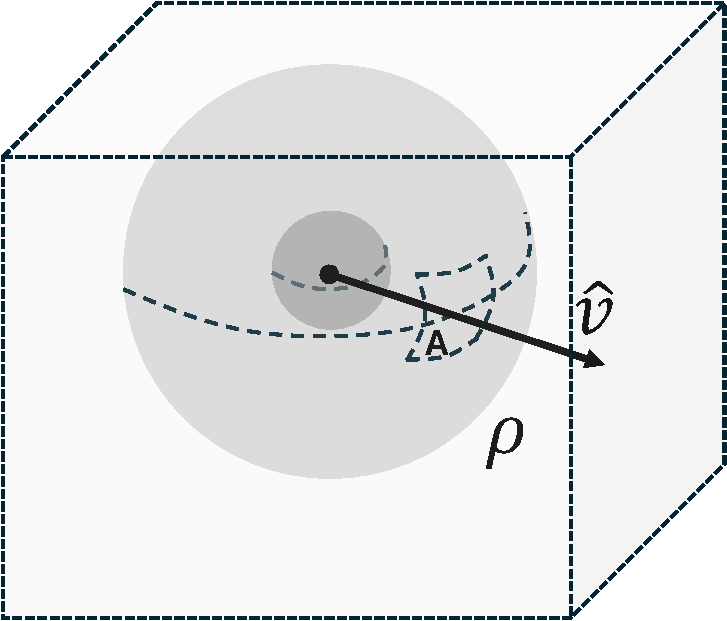
\includegraphics[width=0.3\textwidth]{Chapters/Figures/Ch2_UltrasoundFundamentals/sphere.pdf}
         \caption{$y=x$}
         \label{fig:ch2_spherical_wave}
     \end{subfigure}
     \hfill
     \begin{subfigure}[h]{0.3\textwidth}
         \centering
         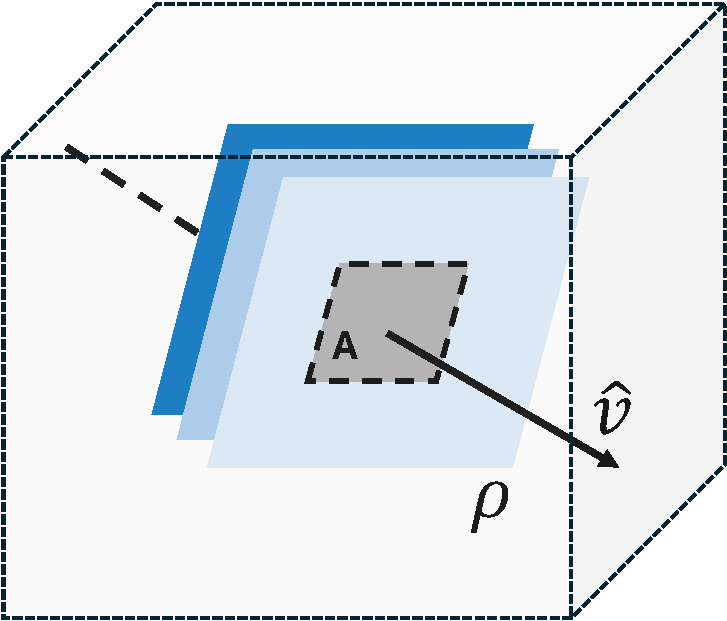
\includegraphics[width=0.3\textwidth]{Chapters/Figures/Ch2_UltrasoundFundamentals/planar.pdf}
         \caption{$y=3\sin x$}
         \label{fig:ch2_planar_wave}
     \end{subfigure}
        \caption{Three simple graphs}
        \label{fig:ch2_wavefront}
\end{figure}

The two most important wave shapes for the aforementioned imaging and stimulation modalities 
are *planar* and *spherical*. Greater focus will be given to a planar wave propagating 
in the media in the following chapters, as it is the fundamental mechanism through 
which the modalities of USI discussed in this work are performed.
A source radiating a mechanical wave from a center point will lead to a spherical wavefront 
propagating with a velocity $v$ in a medium with a density $\rho$ ((Fig. \ref{fig:ch2_spherical_wave})). 
Each wave can be decomposed into sequential infinitely extensible wavefronts that are collienar 
(or in other words, parallel) with each other - just like the ripples observed in the water 
after throwing a rock into a pond. As a single wavefront moves away from the source,
the radius of the spherical surface defining this wavefront grows. An observer interacting 
with this wavefront at an infinite distance away from the source will observe no curvature 
in the wavefront - the velocity vector will be observed/sensed with the same phase in 
all the (square) finite elements in which the wavefront can be decomposed in. In this case 
the wavefront features a planar vectorial velocity field (Fig. \ref{fig:ch2_planar_wave}).
Uppon interacting with an observing particle or *scatterer* in the medium, a *force* will be exerted on it. 
This force is directly proportional to the variation of momentum ($d\hat{\gamma} / dt$) and inversely 
proportional to the area ($A$) of the region in which this variational of momentum is observed. The 
ratio between the exerted force on the observer and the area of the obsrever's surface interacting wit 
the wavefront defines the pressure $p$ this same observer will be subjected to.


\subsection{Mechanical Wave Equation in Fluids}
\label{subsec:ch2_2_mechanical_wave_equation}

As the target application of this dissertation is a medical imaging modality, it is 
important to take an in depth look at the underlying physical phenomena explaining the 
interactions briefly described in the previous subsection for fluids. Most of the \textit{in-vivo} 
setups in which the target applications' scope fits into relies on the propagation of US waves 
in materials best-modelled by incompressible fluids - water, blood, soft tissue, brain 
tissue, muscle and fat. 

In an ideal incompressible fluid, a particle is \textbf{displaced} ($\textbf{u}$)
with a velocity $\textbf{v}$ when a wavefront propagates through a fluid
with a resting-density $\rho$ (\ref{eq:ch2_velocity}).

\begin{equation}
  \textbf{v} = \frac{d \textbf{u}}{dt}
\label{eq:ch2_velocity}
\end{equation}

A velocity \textit{potential} (vectorial field) between any point 
within the medium can be defined for convenience 
(\ref{eq:ch2_velocity_potential}).

\begin(equation)
  \textbf{v} = \nabla \phi
  \label{eq:ch2_velocity_potential}
\end{equation}

The pressure $p$ to which any particle is subjected to 
is then defined by (\ref{eq:ch2_pressure}).

\begin(equation)
  p = -\rho \frac{\partial \phi}{\partial t}
  \label{eq:ch2_pressure}
\end{equation}

The generalized wave equation describbing the propagation of sound 
in an incompressible fluid can then be defined through (\ref{eq:ch2_wave_equation}).

\begin{equation}
  \nabla \textbf{v} - \frac{1}{c^2} \frac{\partial^2 \phi}{\partial t^2} = 0 \equiv \\ 
  \equiv \nabla^2\phi - \frac{1}{c^2} \frac{\partial^2 \phi}{\partial t^2} = 0
  \label{eq:ch2_wave_equation}
\end{equation}

When a wave is propagating in the medium, 
the wave equation enables us find to find regions 
of local pressure disturbance, with higher pressure 
\textit{compressional} regions and - since the fluid is incompressible - 
lower pressure \textit{rarefactional} regions 
(Fig. \ref{fig:ch2_rarefaction_compression}). 
These regions arise from the displacement of particles 
within the fluid, and can occur in the collinear (Fig. \ref{fig:ch2_longitudinal} - longitudinal waves) or 
orthogonal (Fig. \ref{fig:ch2_transversal} - transversal) axis relative to the source of the US waves.


\begin{figure}[ht]
     \centering
     \begin{subfigure}[b]{0.3\textwidth}
         \centering
         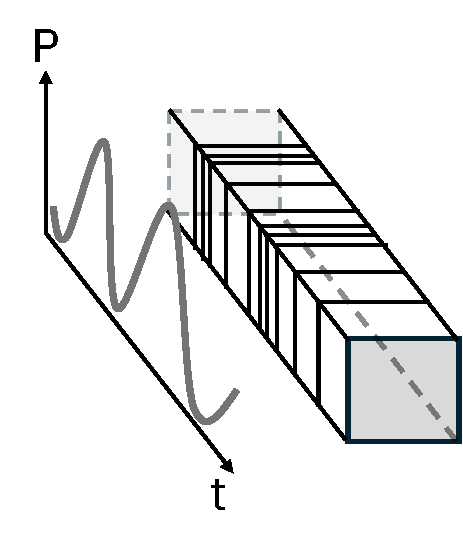
\includegraphics[width=0.3\textwidth]{Chapters/Figures/Ch2_UltrasoundFundamentals/longitudinal_wave.pdf}
         \caption{$y=x$}
         \label{fig:ch2_longitudinal}
     \end{subfigure}
     \hfill
     \begin{subfigure}[b]{0.3\textwidth}
         \centering
         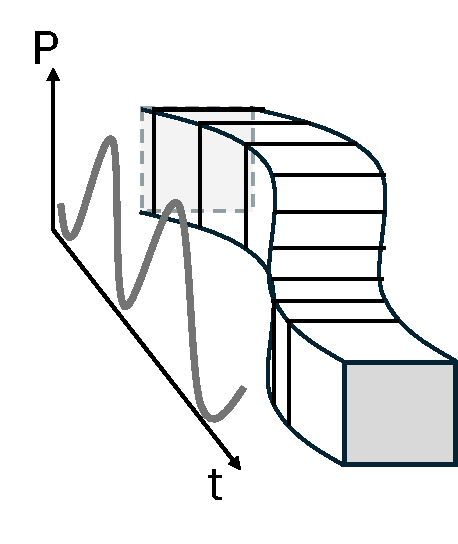
\includegraphics[width=0.3\textwidth]{Chapters/Figures/Ch2_UltrasoundFundamentals/transversal_wave.pdf}
         \caption{$y=3\sin x$}
         \label{fig:ch2_transversal}
     \end{subfigure}
        \caption{Three simple graphs}
        \label{fig:ch2_elastic_waves}
\end{figure}

\subsection{Characteristic Acoustic Impedance and Elastic Wave Propagation}
\label{subsec:ch2_3_propagation}

In a contained volumetric medium, the propagation of an elastic (sound) wave 
in an incompressible liquid medium bounded by elastic boundary surface is 
well-modeled through a longitudinal wave propagating through the liquid. 
In such an environment, the higher the (particle/matter) density of the medium ($\rho$), 
the faster a sound wave can propagate through it with a speed $c_L$.

Any particle travelling within the medium features some \textit{impedance} 
to its displacement. The ratio of pressure ($p$) of the mechanical wave displacing it to the 
particle's velocity ($v_L$) defines the \textit{acoustic characteristic impedance} ($Z$) of 
the medium (\ref{eq:ch2_characteristic_impedance}). 
A more useful definition of medium's $Z$ - in the context of sound propagation - can be 
given through the product of the medium's 
density and the speed of sound in it.

\begin{equation}
  Z = p/v_L = \rho \ c_L \ \mathrm{[Rayl \equiv kg/m^2s]}
  \label{eq:ch2_characteristic_impedance}
\end{equation}

The propagation of a sound wave between two media with different acoustic chatacteristic 
impedances $Z_1,Z_2$ and sound velocities $c_1, c_2$ is conditioned by two phenomena - \emph{reflection} and \emph{diffraction} (Fig. \ref{fig:ch2_reflection_diffraction}). 
Diffraction is describbed using an equivalent of 
Snell's Law for elastic waves (\ref{eq:ch2_diffraction}). 

\begin{equation}
  \frac{\sin{\theta_{11}}}{\sin{\theta_{21}}} = \frac{c_1}{c_2}
  \label{eq:ch2_diffraction}
\end{equation}

\begin{figure}[h]{0.5\textwidth}
  \begin{subfigure}[b]{0.4\textwidth}
      \centering
      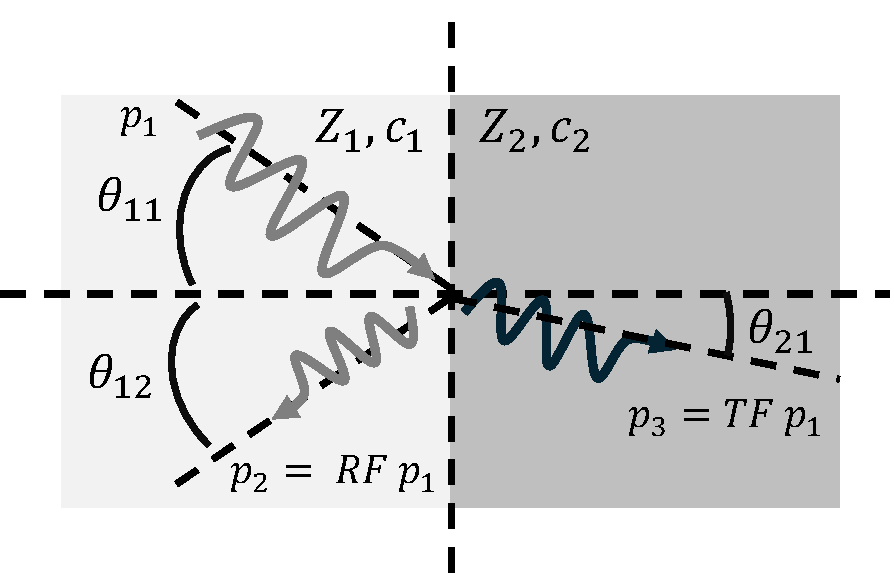
\includegraphics[width=0.4\textwidth]{Chapters/Figures/Ch2_UltrasoundFundamentals/reflection_diffraction.pdf}
      \label{fig:ch2_reflection_diffraction}
  \end{subfigure}
  \hfill
  \begin{subfigure}[b]{0.4\textwidth}
      \centering
      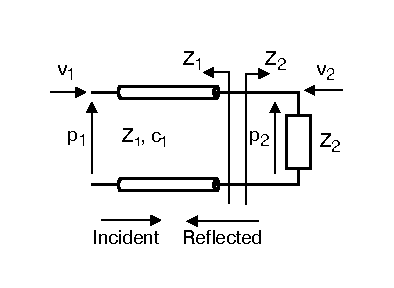
\includegraphics[width=0.4\textwidth]{Chapters/Figures/Ch2_UltrasoundFundamentals/impedance_schematic.pdf}
      \label{fig:ch2_dynamic_range}
  \end{subfigure}
     \caption{Three simple graphs}
     \label{fig:ch2_elastic_waves}
\end{figure}

The mismatch (dissimilarity) 
between acoustic characteristic impedances determines the magnitude of the reflected wave, 
where the reflected wave features the same angle as the incident wave (Fig. \ref{fig:ch2_reflection}). 
As in electromagnetic wave propagation, the \textit{reflection factor} ($RF$) can be defined - through the 
analysis of the propagation between media as a two-port propagation problem - to determine \textit{how much} 
of the incident wave's energy \textit{is reflected back into medium 1} (\ref{eq:ch2_reflection_factor}). 
Similarly, the \textit{transmission factor} ($TF$) is defined as the energy ratio of the signal that is 
transmitted between the two media (\ref{eq:ch2_transmission_factor}), linearly proportional to $RF$ - if RF grows in 
magnitude, TF will innevitably reduce in magnitude as well by the same proportion.

\begin{equation}
  RF = \frac{Z_2 - Z_1}{Z_2 + Z_1}
  \label{eq:ch2_reflection_factor}
\end{equation}

\begin{equation}
  TF = \frac{2 \ Z_2}{Z_2 + Z_1}
  \label{eq:ch2_transmission_factor}
\end{equation}

\begin{figure}[h]{1.0\textwidth}
    \centering
  \begin{subfigure}[b]{0.4\textwidth}
      \centering
      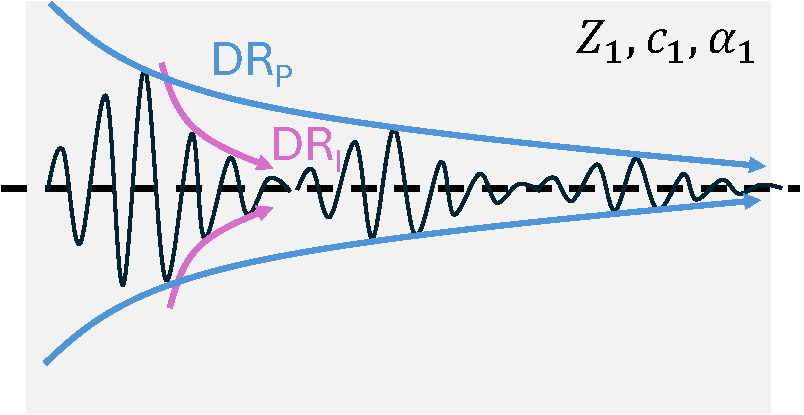
\includegraphics[width=0.4\textwidth]{Chapters/Figures/Ch2_UltrasoundFundamentals/attenuation.pdf}
      \label{fig:ch2_attenuation}
  \end{subfigure}
  \hfill
  \begin{subfigure}[b]{0.4\textwidth}
      \centering
      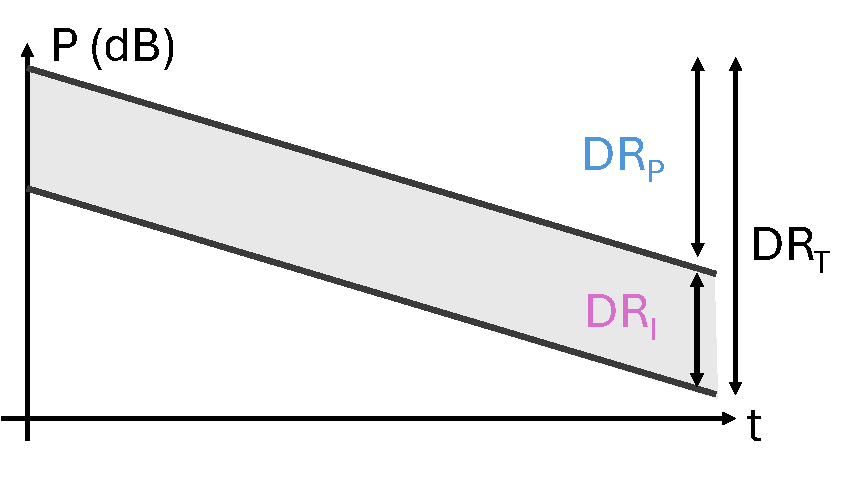
\includegraphics[width=0.4\textwidth]{Chapters/Figures/Ch2_UltrasoundFundamentals/dynamic_range.pdf}
      \label{fig:ch2_dynamic_range}
  \end{subfigure}
     \caption{Three simple graphs}
     \label{fig:ch2_elastic_waves}
\end{figure}

\emph{Attenuation} is the governing phenomena leading to the progressive loss of energy of an elastic wave 
propagating in any media - mainly due to \emph{energy scattering} and \emph{energy absorption} phenomena intrinsic to the 
incompressible liquid(s) constituing the media (Fig. \ref{fig:ch_attenuation}). % https://en.wikipedia.org/wiki/Attenuation#cite_note-10 
While \emph{absorption} is the main factor in the propagation of an elastic wave in an \emph{homogeneous medium}, 
\emph{scattering} should also be taken into account for \emph{heterogeneous} media - \emph{i.e.} the human body. In diagnostic US applications 
it is often the case that the sonicated volumetric regions are relatively small, enabling soft tissue regions of the body 
to be well approximated by an homogeneous medium. Attenuation through absorption becomes then the main 
issue to address when developping readout systems for diagnostic US. Attenuation 
of an acoustic wave propagating within a medium ($DR_P$ in dB) is linear-in-dB, and is represented by an exponent power factor that is directly proportional to 
the center frequency of the carrier of the wave ($f_0$ in $MHz$), the \emph{roundtrip} distance the wave (and in diagnostic US, its corresponding echo) 
travels ($D_L$ in $cm$) and the attenuation coefficient of the material it propagates in ($\alpha$ in $dB MHz^{-1} cm^{-1}$) (\ref{eq:ch2_propagation_dyn_range}). 
Throughout this thesis, this propagation-induced attenuation ($DR_P$) is also referred to as \emph{propagation dynamic range}. 
US waves can be decomposed into a superposition of vector-basis functions that are gaussian-modulated cosine 
temporal impulse responses \cite{}. Each gaussian distribution modulating the center tone has a 6-dB pass-band bandwidth 
that most often creates a 40 dB \emph{instantaneous dynamic range} ($DR_I$) on the impulse response of 
any low Q-factor, wide-bandwidth transducer preferable in most diagnostic US applications \cite{} (Fig. \ref{fig:ch2_dynamic_range}). Superposed 
to $DR_P$, the \emph{total dynamic range} ($DR_T$) of a typical US echo verified in most diagnostic US applications can range 
from 60 dB to 120 dB. \emph{instantaneous dynamic range} and other transducer-related concepts are 
further discussed in Sec. \ref{sec:ultrasound_transducers} with a greater depth.

\begin{equation}
  DR_P = f_0 \ D_L \ \alpha \ \mathrm{[dB \ MHz^{-1} \ cm^{-1}]}
  \label{eq:ch2_propagation_dyn_range}
\end{equation}

\begin{equation}
  DR_T = DR_P + DR_I \ \mathrm{[dB]}
  \label{eq:ch2_propagation_dyn_range}
\end{equation}

Common bio-materials found within the body 
of mammals feature attenuation coefficients 
typically leading to 30 - 60 dB of 
\emph{propagation dynamic range}. The attenuation 
coefficients of such bio-materials can be found in 
table \ref{tab:ch2_attenuation_coefs}.

\begin{table}[!ht]
    \centering
    \caption{Attenuation coefficients for commonly found biological mediums in the body of mammals \cite{Culjat2010uim\&b}}
    \begin{longtable}{lc}
        Medium & Attenuation ($\alpha$) [$dB \ MHz^{-1} \ cm^{-1}$] \\ \hline
        Air & 1.64 \\ 
        Water & 0.0022 \\ 
        Blood & 0.2 \\ 
        Bone (Cortical) & 6.9 \\ 
        Bone (Trabecular) & 9.94 \\ 
        Brain & 0.6 \\ 
        Breast & 0.75 \\ 
        Cardiac & 0.52 \\ 
        Connective Tissue & 1.57 \\ 
        Fat & 0.48 \\ 
        Marrow & 0.5 \\ 
        Muscle & 1.09 \\ 
        Tendon & 4.7 \\ 
        Soft Tissue (Average) & 0.54 \\ 
    \end{longtable}
    \label{tab:ch2_attenuation_coefs}
\end{table}

\section{Ultrasound Transducers}
\label{sec:ultrasound_transducers}

In this section, the fundamental concepts enabling the 
representation of the US trasnducer in the electrical 
domain are described. The electrical modelling of 
any trasnducer geometry and material is fundamental to 
optimize the design of \emph{unipolar} and \emph{multipolar} 
drivers in \emph{therapeutic} US. An accurate electrical impedance 
modelling of the trasnducer also enables the optimization 
of \emph{DC-decoupling} and \emph{input impedance} matching networks 
in the \emph{low-noise amplifier} (LNA) located at the interface 
between the transducer and the AFE.



The \emph{Butterworth-van-Dyke} (BVD) model \cite{VanDyke1928poti} (Fig. \ref{fig:ch2_bvd_model}) is a simplification of the 
Krimholtz, Leedom, and Matthaei (KLM) model \cite{Leedom1971itosau} considering the latter is operated as 
a resonating network. While the KLM model is a complete two-port model allowing for the bidirectional 
direct translation between the 
acoustic pressure interfacing with the piezoelectric transducer's surface and the electric potential within 
the top and bottom plate, the BVD model outputs an electrical output from the electrical input 
equivalent to a generated \emph{displacement current} ($I_d$) or \emph{displacement voltage} ($V_d$).
Such a transformation in analysis-domain greatly simplifies the electrical modelling 
of the piezoelectric model from a pre-characterization process of its \emph{charge-displacement} 
system matrix representation \cite{Szabo2014duiioTransducers}. The BVD model includes a resonant 
branch ($R_m$ , $L_m$ , $C_m$ ) modelling the mechanical resonance of the transducer, and a parasitic capacitor 
($C_p$ ) representing the electrical losses dampening the resonator branch over time Fig. \ref{fig:ch2_bvd_model}).

\begin{figure}
  \centering
  \begin{subfigure}[][][t]{0.3\textwidth}
      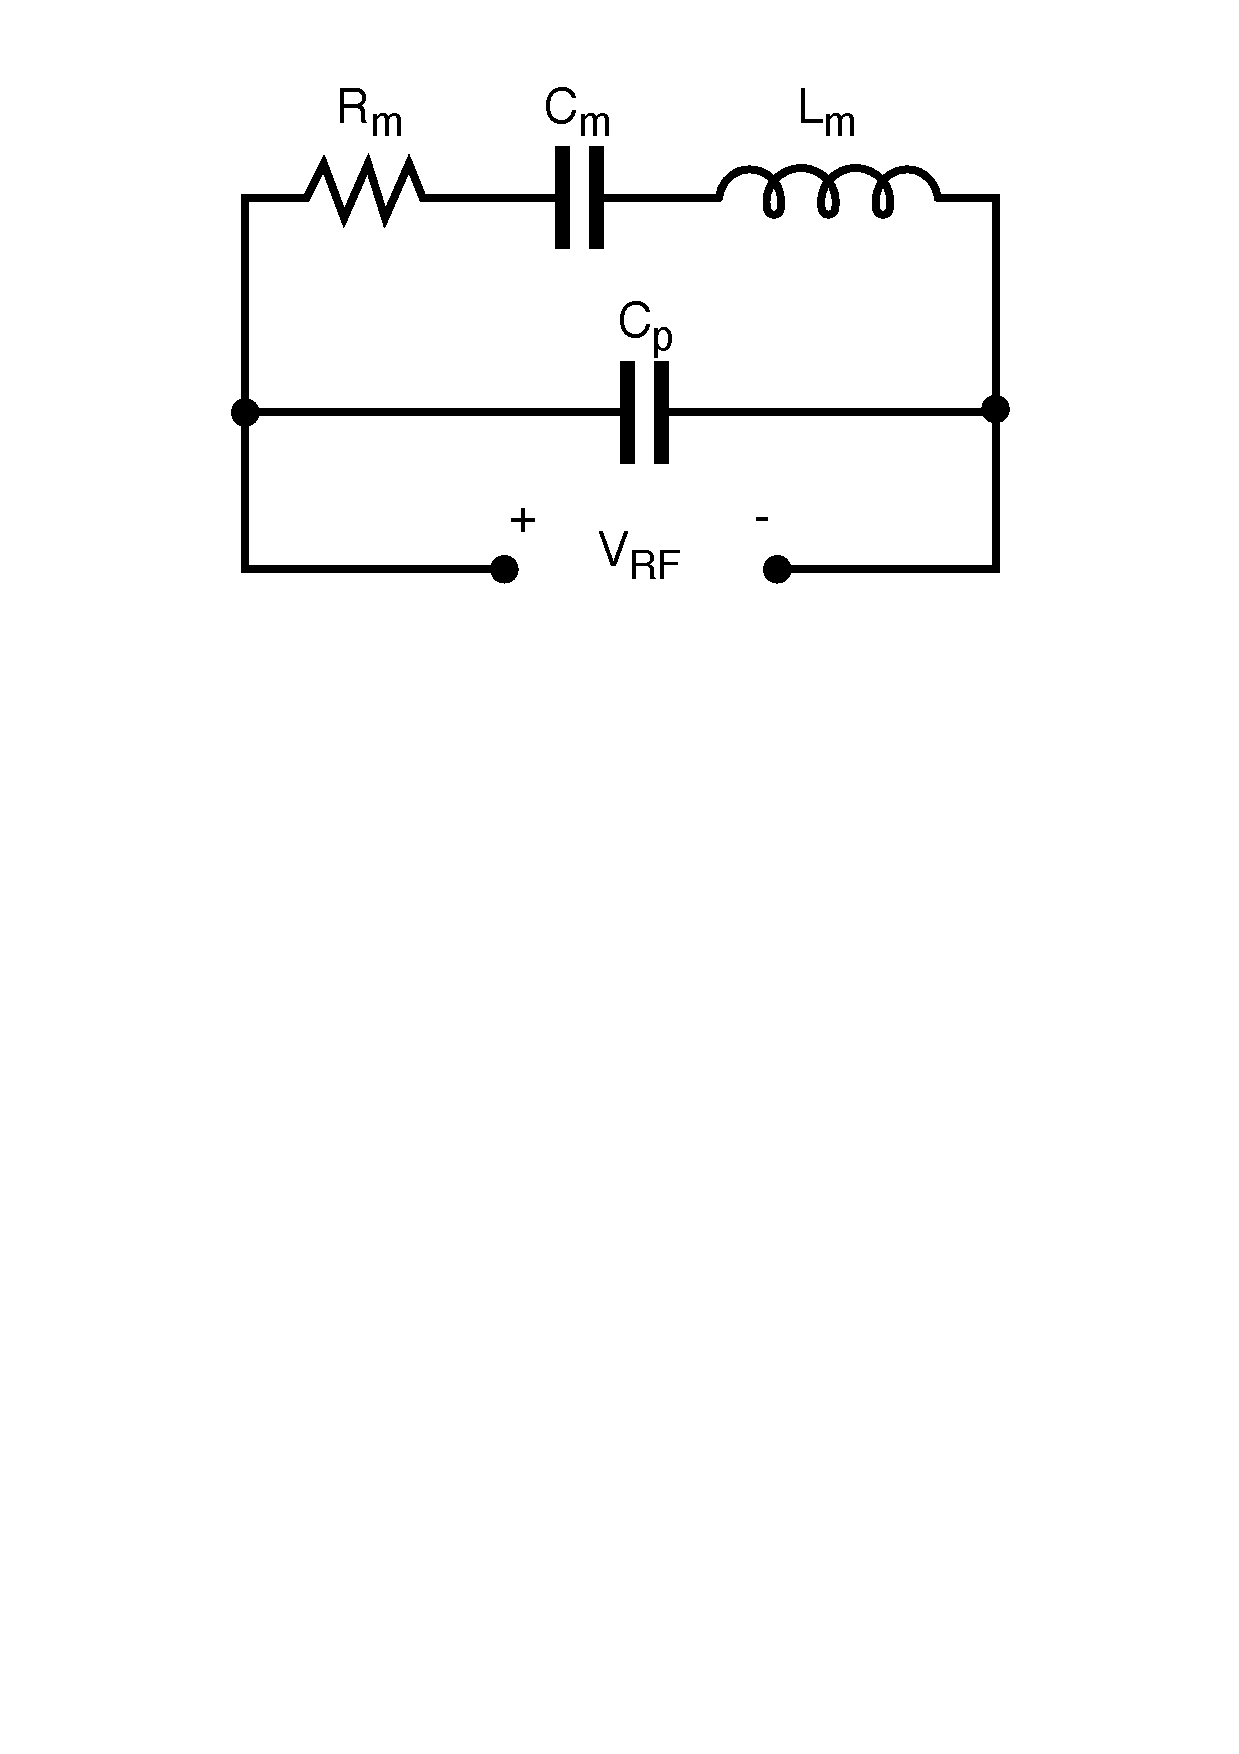
\includegraphics[width=0.45\textwidth]{Chapters/Figures/Ch2_UltrasoundFundamentals/bvd_model.pdf}
      \label{fig:ch2_bvd_model}
  \end{subfigure}
  %\hfill
  \begin{subfigure}[][][t]{0.3\textwidth}
      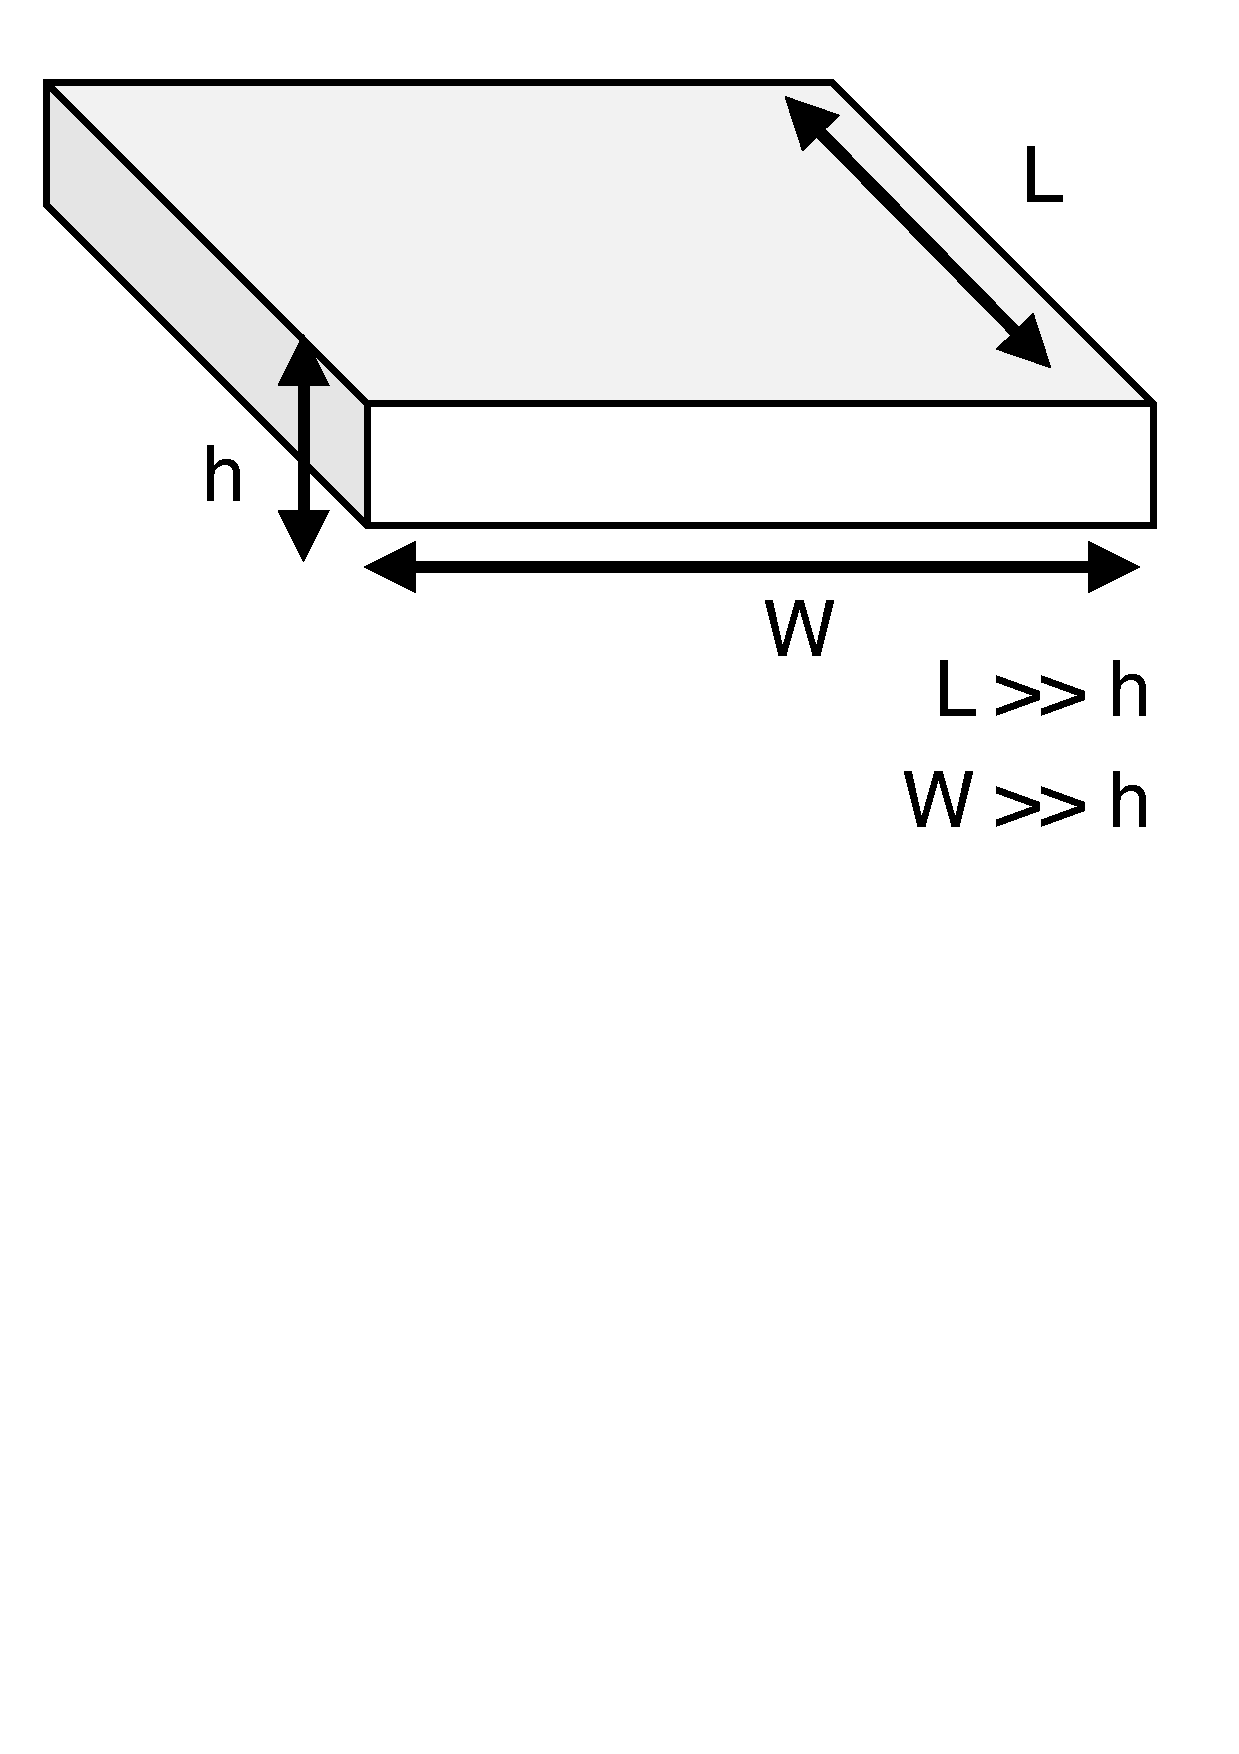
\includegraphics[width=0.45\textwidth]{Chapters/Figures/Ch2_UltrasoundFundamentals/planar_piezo.pdf}
      \label{fig:ch2_planar}
  \end{subfigure}
  %\hfill
  \begin{subfigure}[][][b]{0.3\textwidth}
      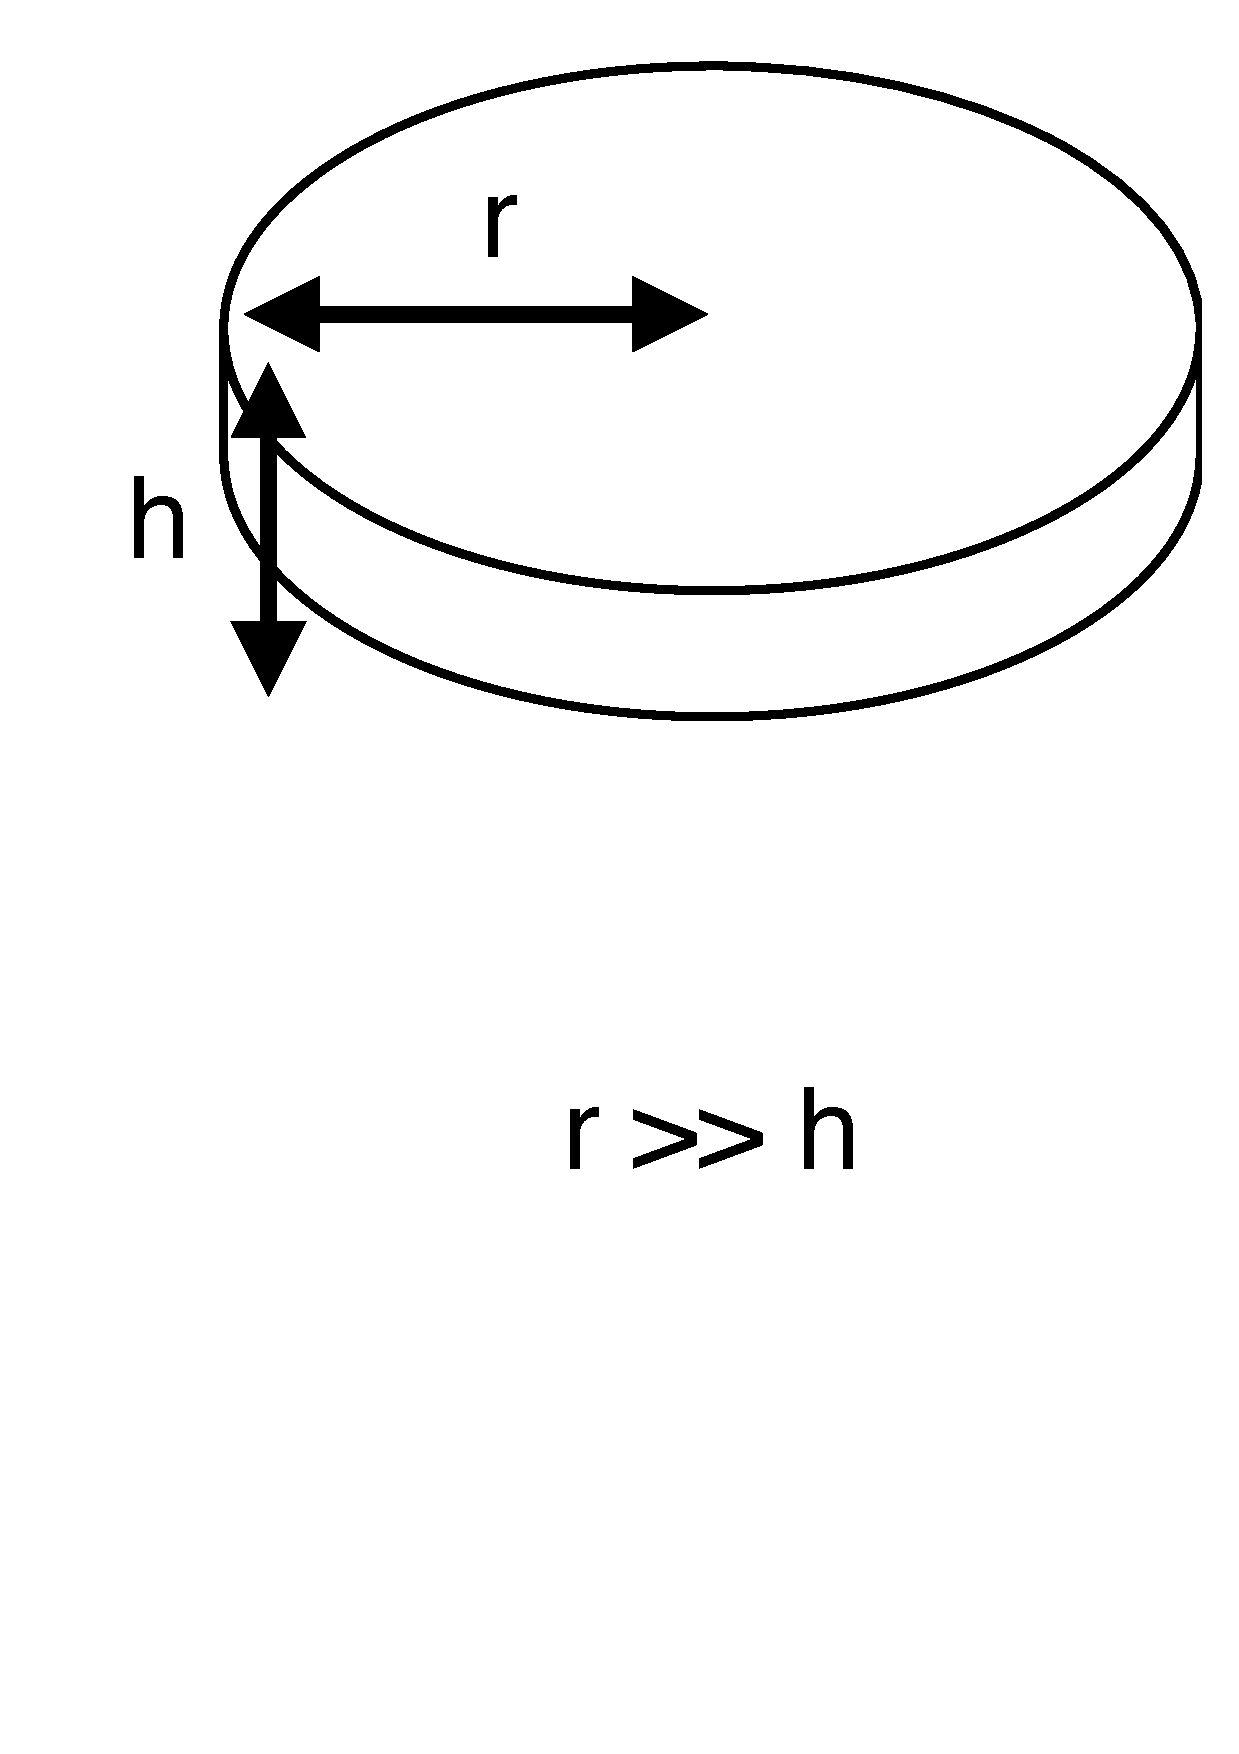
\includegraphics[width=0.45\textwidth]{Chapters/Figures/Ch2_UltrasoundFundamentals/cilinder_piezo.pdf}
      \label{fig:ch2_cillinder}
  \end{subfigure}
  %\hfill
  \begin{subfigure}[][][b]{0.3\textwidth}
      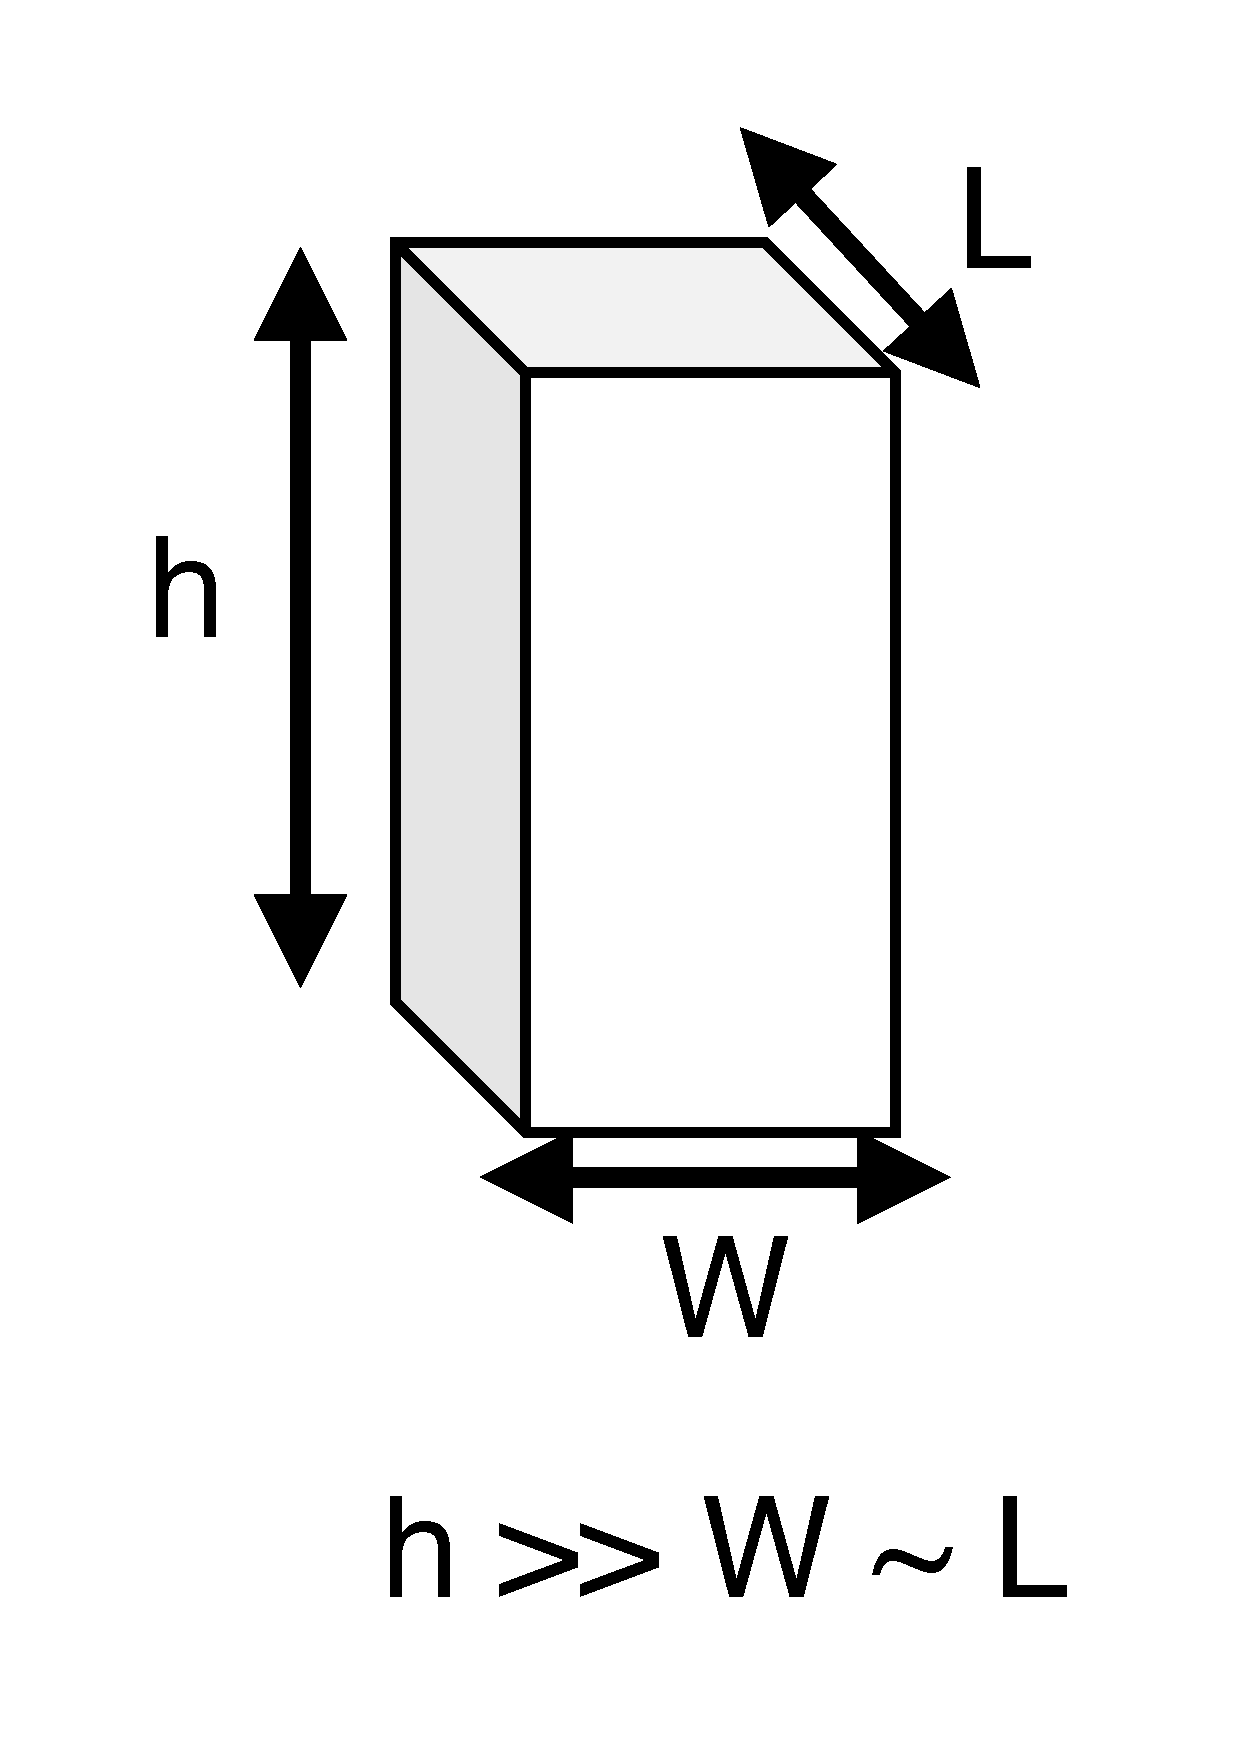
\includegraphics[width=0.45\textwidth]{Chapters/Figures/Ch2_UltrasoundFundamentals/pillar_piezo.pdf}
      \label{fig:ch2_pillar}
  \end{subfigure}
  %\hfill
  \begin{subfigure}[][][b]{0.3\textwidth}
      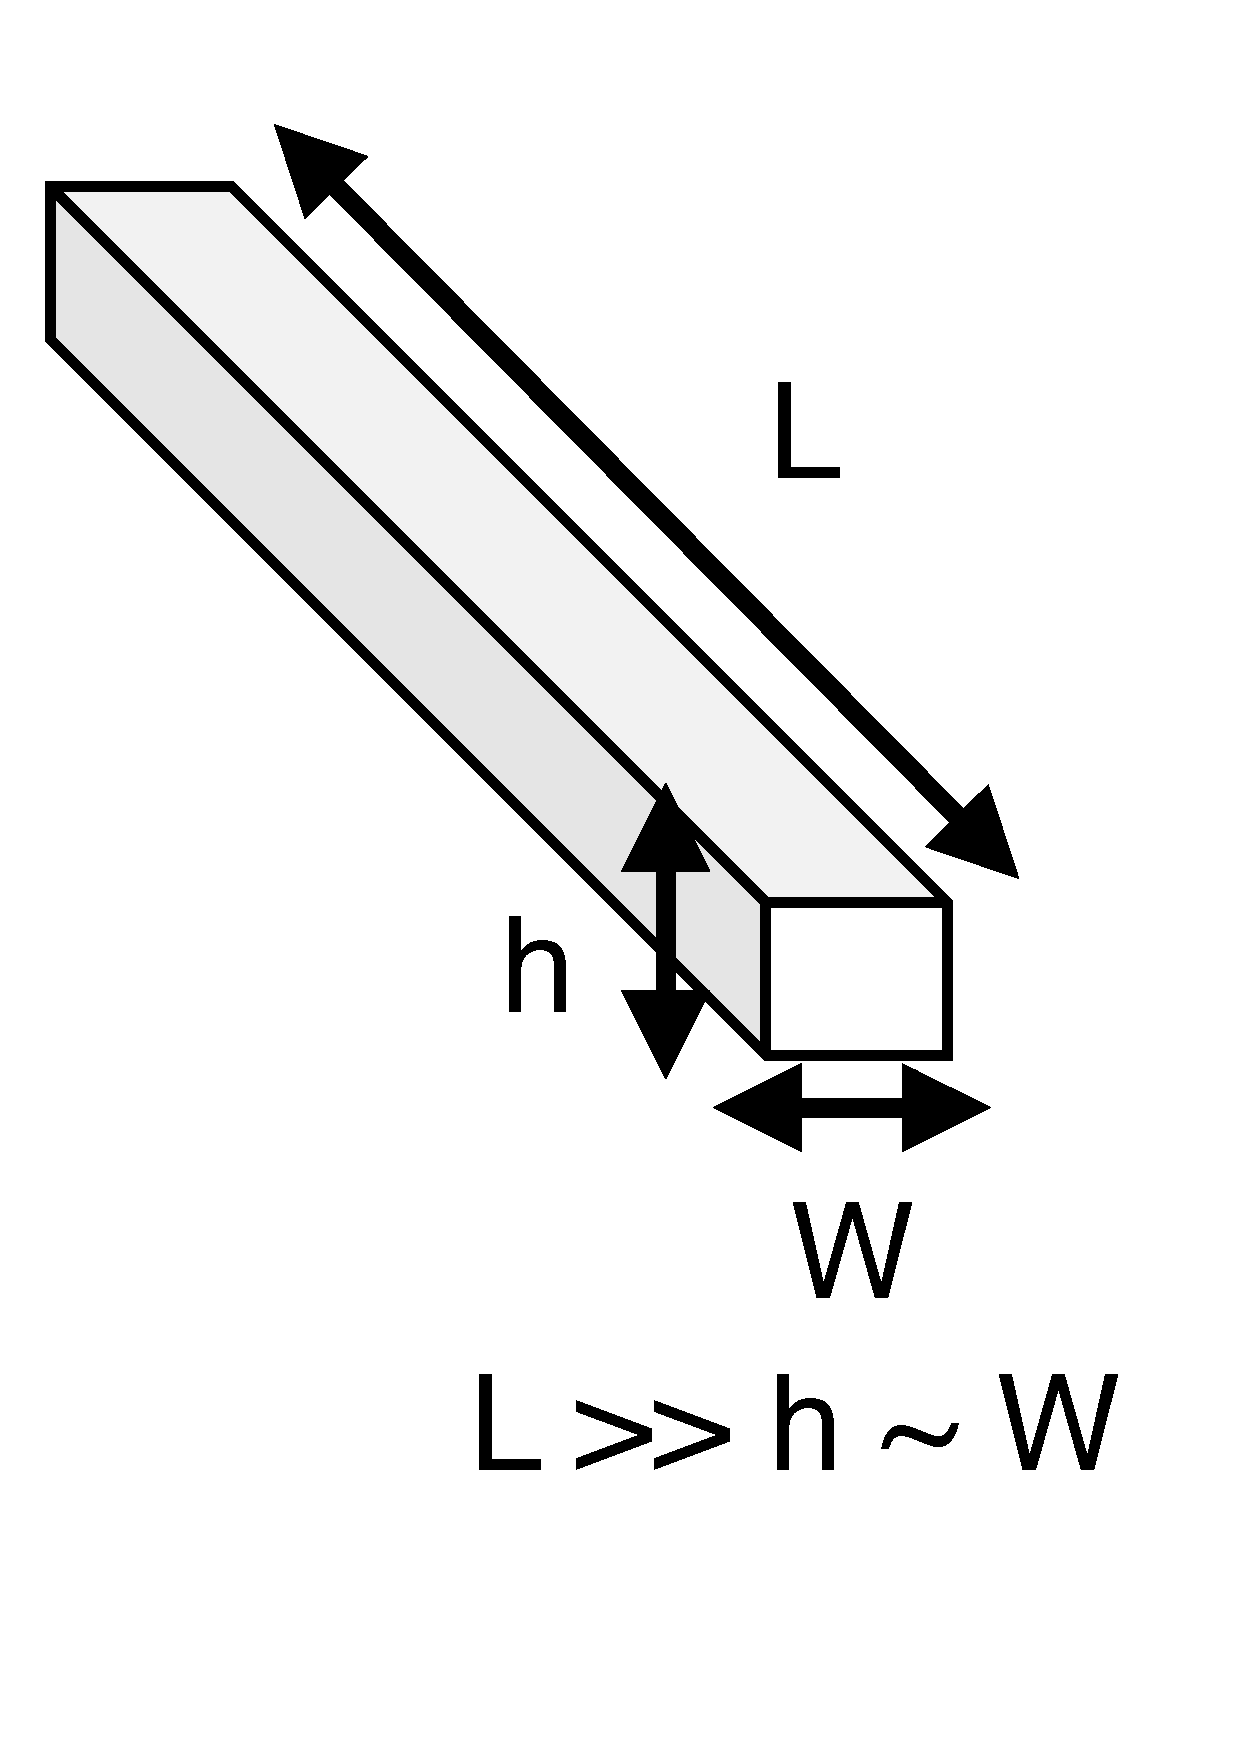
\includegraphics[width=0.45\textwidth]{Chapters/Figures/Ch2_UltrasoundFundamentals/horiz_pillar_piezo.pdf}
      \label{fig:ch2_h_pillar}
  \end{subfigure}

  \caption{Creating subfigures in \LaTeX.}
  \label{fig:ch2_bvd_model_and_transducer_types}
\end{figure}



\begin{equation}
  Q = f_0 / BW
  \label{eq:q_factor}
\end{equation}



\section{Therapeutic \& Diagnostic Ultrasound}
\label{sec:ultrasound_imaging}

The pressure generated at the surface of the elements depends on the 
amplitude of the applied pulse, and the transmit efficiency (expressed in Pa/V) 
of the transducer. In the case of focused transmission, the pulses are timed by 
the transmit beamformer such that the gen- erated acoustic waves converge at the 
desired focal point. The pressure at this focal point can then be found by taking 
into account the TX beamforming gain and the propagation attenuation in the medium. 

The acoustic wave will reflect from interfaces between regions with different 
acoustic impedance in the medium, leading to echoes that return to the transducer. 
The amplitude of an echo depends on the reflection coefficient associated with the 
interface, and the geometrical spreading and atten- uation that the echo experiences 
as it travels back to the transducer. The resulting surface pressure at one of the 
elements then translates to a voltage through the trans- ducer’s receive sensitivity 
(expressed in V/Pa). This signal is amplified by the LNA and TGC and digitized, and 
finally combined with the signals from other elements by the receive beamformer. 
Upon performing delay-and-sum (DAS), the correlated signals from the different channels 
add up constructively, while uncorrelated noise does not, giving an RX beamforming gain 
and leading to the creation of a pressure profile through time, leading to the reconstruction 
of an US B-mode image upon quadrature-filtering and log-compression of the beamformed RX US 
signals.



% \section{Compressive Sensing in Diagnostic Ultrasound} % - Introduce in State of the Art